% !TeX document-id = {0be8c18c-9430-4e9a-bdd9-12beadebfebc}
% !TeX TXS-program:bibliography = txs:///biber
\documentclass[11pt]{beamer}

\usepackage[brazilian]{babel}

\uselanguage{portuguese}
\languagepath{portuguese}
\deftranslation[to=portuguese]{Theorem}{Teorema}
\deftranslation[to=portuguese]{theorem}{teorema}
\deftranslation[to=portuguese]{Example}{Exemplo}
\deftranslation[to=portuguese]{example}{exemplo}
\deftranslation[to=portuguese]{Lemma}{Lema}
\deftranslation[to=portuguese]{lemma}{Lema}
\deftranslation[to=portuguese]{Corollary}{Corolário}
\deftranslation[to=portuguese]{corollary}{corolário}
%\deftranslation[to=portuguese]{and}{e}


\usepackage[utf8]{inputenc}
\usepackage[T1]{fontenc}
\usepackage{lmodern}
\usepackage{amsmath}
\usepackage{amssymb}
\usepackage{mathtools}
\usepackage{color}
\usepackage{pgfplots}
\usepackage{tikz}
\usepackage{subcaption}
%\usepackage{appendixnumberbeamer}

\newenvironment{transitionframe}{
	\setbeamercolor{background canvas}{bg=yellow}
	\begin{frame}}{
	\end{frame}
}
\usetheme{default}
\usefonttheme{structuresmallcapsserif}

%% I use a beige off white for my background
\definecolor{MyBackground}{RGB}{255,253,218}
\useinnertheme[shadow]{rounded}
\setbeamercolor{block title}{bg=MyBackground}
\setbeamercolor{block body}{bg=MyBackground}
\setbeamercolor{example title}{bg=MyBackground}
\setbeamercolor{example body}{bg=MyBackground}


\newcommand{\blue}[1]{\textcolor{blue}{#1}}
\newcommand{\red}[1]{\textcolor{red}{#1}}
\newcommand{\purple}[1]{\textcolor{purple}{#1}}
\newcommand{\gray}[1]{\textcolor{gray}{#1}}
\setbeamertemplate{navigation symbols}{}
%\setbeamertemplate{page number in head/foot}[appendixframenumber]

%\usepackage{graphics}
\usepackage{graphicx}

\definecolor{blue_emph}{RGB}{0,114,178}
\definecolor{red}{RGB}{213,94,0}
\definecolor{yellow}{RGB}{240,228,66}
\definecolor{green}{RGB}{0,158,115}
\definecolor{purple}{RGB}{204,121,167}
\definecolor{orange}{RGB}{230,159,0}
\definecolor{lightblue}{RGB}{86,180,233}

%\setbeamercolor{frametitle}{fg=blue}
%\setbeamercolor{title}{fg=blue}
\setbeamertemplate{footline}[frame number]
\setbeamertemplate{navigation symbols}{} 
\setbeamertemplate{itemize items}{-}
%\setbeamercolor{itemize item}{fg=blue}
%\setbeamercolor{itemize subitem}{fg=blue}
\setbeamertemplate{enumerate items}[default]
%\setbeamercolor{enumerate subitem}{fg=blue}
\setbeamercolor{button}{bg=MyBackground,fg=blue}
\usefonttheme{structuresmallcapsserif}

%\setbeamercolor{section in toc}{fg=blue}
%\setbeamercolor{subsection in toc}{fg=red}
\setbeamersize{text margin left=1em,text margin right=1em} 


\usepackage{appendixnumberbeamer}

\usepackage[
backend=biber,
uniquename=false,
uniquelist=false,
style=authoryear,
natbib=true
]{biblatex}
\addbibresource{../bibliography.bib}

\newenvironment{wideitemize}{\itemize\addtolength{\itemsep}{10pt}}{\enditemize}
\newenvironment{wideenumerate}{\enumerate\addtolength{\itemsep}{10pt}}{\endenumerate}
\newenvironment{halfwideitemize}{\itemize\addtolength{\itemsep}{0.5em}}{\enditemize}
\newenvironment{halfwideenumerate}{\enumerate\addtolength{\itemsep}{0.5em}}{\endenumerate}


\author{Luis A. F. Alvarez}
\title{EAE1223: Econometria III}
\subtitle{Aula 7 - Cointegração}
%\logo{}
%\institute{}
\date{\today}
%\subject{}
%\setbeamercovered{transparent}

\begin{document}

\begin{frame}[plain]
	\maketitle
\end{frame}

\begin{frame}{Natureza da inferência espúria}
	\begin{wideitemize}
		\item Em algumas aulas atrás, vimos que a inferência baseada nos estimadores de MQO de um modelo linear de um processo I(1) em outro processo I(1), {\color{blue} completamente independentes}, gerava conclusões espúrias.
		\begin{itemize}
			\item Relação verdadeira é $0$, mas testes de hipótese proviam forte evidência contra hipótese de associação nula  (p-valores baixíssimos).
		\end{itemize}
		\item Uma pergunta que cabe é: se há dependência entre os processos I(1), há condições sob as quais estimadores de MQO produzem inferência \textbf{não espúria}? 
	\end{wideitemize}

\end{frame}

\begin{frame}{Um exemplo}
	\begin{itemize}
		\item Considere o seguinte processo bivariado :
		$$x_t =  x_{t-1}+u_t \, ,$$
		$$ y_t = \gamma x_t + v_t\, ,$$
		onde $\{u_t\}_t$ e $\{v_t\}_t$ são ruídos brancos independentes uns dos outros.
		\item Observe que ambos os processos são I(1)
		\item Vamos considerar as propriedades do estimador de MQO $\hat \gamma$  de $\gamma$, sobre realizações repetidas da incerteza econômica:
	\end{itemize}
\end{frame}

\begin{frame}{Uma realização do processo por $T=500$ períodos ($\gamma =0.5$)}
\begin{figure}
	\centering
	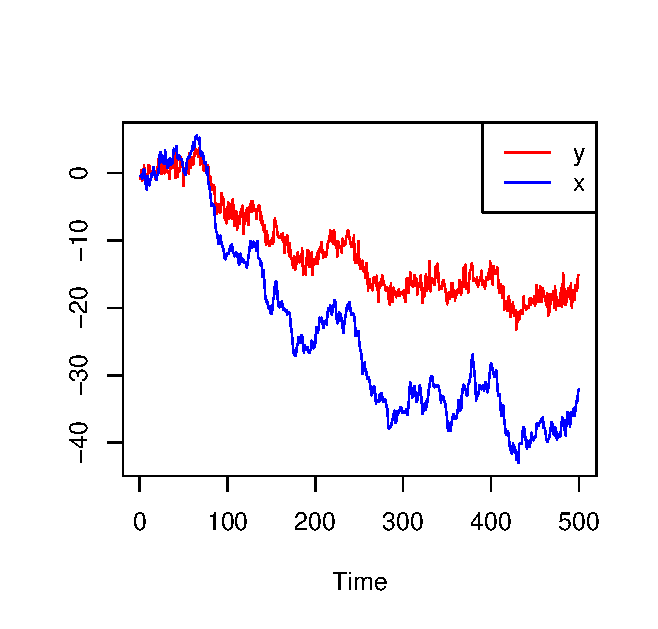
\includegraphics[scale=0.7]{graficos/tendencia_comum.pdf}
\end{figure}
\end{frame}

\begin{frame}{Distribuição de $\hat t = \frac{\hat \gamma - \gamma}{\operatorname{se}(\hat \gamma)}$ em realizações repetidas da incerteza ($T=500$  e $\gamma =0.5$)}
\begin{figure}
	\centering
	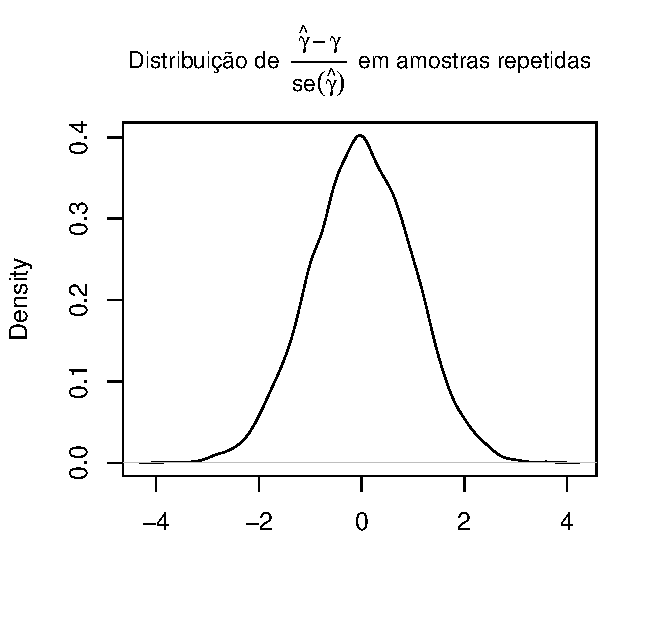
\includegraphics[scale=0.7]{graficos/distribuicao_that.pdf}
\end{figure}
\end{frame}

\begin{frame}{Tendência estocástica comum}
	\begin{itemize}
		\item Note que a estatística $t$, sob a nula, tem distribuição convencional (normal) sobre realizações repetidas da incerteza.
		\item Isso ocorre mesmo com ambas as séries sendo I(1).
		\item Por que isso ocorre?
		\begin{itemize}
			\item Processos possuem tendência estocástica {\color{blue}\textbf{comum}}.
			\item A tendência comum ``amarra'' o comportamento explosivo dos processos, recuperando a validade da aproximação normal.
			\item A processos I(1) com tendência estocástica comum, damos o nome de {\color{blue}processos cointegrados}.
		\end{itemize}
	\end{itemize}
\end{frame}

\begin{frame}{Cointegração}
\begin{itemize}
	\item Considere um processo vetorial $\{\boldsymbol{Z}_t\}_{t \in \mathbb{Z}}$ com $n$ variáveis.
	\item Dizemos que o vetor é cointegrado (de ordem (1,1)), ou CI(1,1), se:
	\begin{enumerate}
		\item Cada uma das séries $\{Z_{jt}\}_{t\in \mathbb{Z}}$, $j=1,\ldots, n$, é I(1).
		\item Existe um vetor $\boldsymbol{\gamma} \in \mathbb{R}^n$, $\boldsymbol{\gamma} \neq \boldsymbol{0}_{n\times 1}$, tal que $\boldsymbol{\gamma}'\boldsymbol{Z}_t$, é I(0).
	\end{enumerate} 
	\item Se processo é CI(1,1), existe combinação linear não trivial tal que processo resultante é estacionário.
	\begin{itemize}
		\item Existe uma {\color{blue}relação de longo prazo}, fruto de uma tendência comum, amarrando os processos, de modo que desvios dessa relação são I(0).
		\item Note que a relação não é única, visto que sempre podemos multiplicá-la por uma constante não nula.
	\end{itemize}
	\item De modo mais geral, um processo vetorial é dito cointegrado de ordem (d,b), ou CI(d,b), $ 0< b \leq  d$, se:
	\begin{itemize}
			\item Cada uma das séries $\{Z_{jt}\}_{t\in \mathbb{Z}}$, $j=1,\ldots, n$, é I(d).
					\item Existe um vetor $\boldsymbol{\gamma} \in \mathbb{R}^n$, $\boldsymbol{\gamma} \neq 0$, tal que $\boldsymbol{\gamma}'\boldsymbol{Z}_t$, é I(d-b).
	\end{itemize}
	\item Focaremos no caso CI(1,1), que é o mais economicamente interessante.
\end{itemize}
\end{frame}

\begin{frame}{Cointegração e teoria econômica}
	\begin{itemize}
		\item O conceito de cointegração é de natureza estatística.
		\begin{itemize}
			\item Não obstante, a evidência ou não de uma relação de longo prazo pode ter uma interpretação econômica.
		\end{itemize}
		\item Considere uma medida dos preços praticados para uma cesta de bens no Brasil, em reais; uma outra medida, para cesta similar, dos preços praticados em dólares nos Estados Unidos, e a taxa de câmbio real/Estados Unidos.
		\begin{itemize}
		\item  {\color{blue}Pela teoria da paridade do poder de compra}, embora processos individualmente apresentem comportamento não estacionário (estocástico), deveria haver uma relação de cointegração entre estas variáveis.
		\end{itemize}
		
		\item {\color{blue}Se há neutralidade da moeda no longo prazo}, \textbf{não} deveria haver relação de longo prazo entre produto real e base monetária \textbf{nominal}; embora devesse haver relação de longo prazo entre produto real e base monetária \textbf{real}.
		
	\end{itemize}
\end{frame}

\begin{frame}{Testando pela presença de cointegração}
	\begin{itemize}
		\item \citet{EngleGranger1987} popularizaram um procedimento bastante intuitivo para se testar a nula de\textbf{ não cointegração}.
		\item Considere um processo vetorial $\boldsymbol{Z}_t = (y_t, \boldsymbol{x}_t)$ em que cada entrada é I(1), e para o qual acreditamos que possa haver alguma relação de cointegração envolvendo $y_t$.\begin{itemize}
			\item Para sistemas com duas variáveis  ($\boldsymbol{x}_t$ escalar), crença é sem perda de generalidade, visto que cointegração necessariamente envolve $y_t$.
			\item Para sistemas com mais de duas variáveis, efetivamente nos restringimos a alternativas em que $y_t$ participa da relação.
		\end{itemize}
		\item Ideia de \citet{EngleGranger1987}: estimar por MQO uma regressão de $y_t$ em $\boldsymbol{x}_t$ (e um intercepto):
		$$y_t =\hat\alpha + \hat{{\gamma}}'\boldsymbol{x}_t + \hat{u}_t \, , \quad t=1,\ldots, T$$
		e fazer um teste da nula de raiz unitária nos resíduos $\{\hat u_t\}_{t=1}^T$.
		\begin{itemize}
			\item Se não há cointegração, resíduos devem apresentar tendência estocástica.
			\item Se há cointegração envolvendo $y_t$, resíduos deveriam ser estacionários.
		\end{itemize}
	\end{itemize}
\end{frame}
\begin{frame}{Procedimento de \citet{Phillips1990}}
	\begin{itemize}
		\item Teste não pode ser feito usando valores críticos convencionais, pois estimação preliminar afeta valores críticos.
		\begin{itemize}
			\item \citet{Phillips1990} tabularam os valores críticos para as estatísticas do teste ADF e de \citet{Phillips1988}.
		\end{itemize}
		\item Tabulação depende de existência de tendência linear no nível da série.
		\begin{itemize}
			\item Se há somente tendência estocástica em nível, usar {\color{blue}Caso 2}.
			\item  Se séries apresentam tendência estocástica, e ao menos uma das séries em $\boldsymbol{x}_t$ apresentar tendência determinística linear em nível, usar {\color{blue}Caso 3}.
			\item Se séries apresentam tendência estocástica, nenhuma das séries em $\boldsymbol{x}_t$ apresentar tendência determinística em nível, mas $y_t$ apresentar tendência linear, há que se modificar o conceito de cointegração. Nesse caso, é impossível gerar combinação linear estacionária, mas ainda é possível gerar combinação linear \textit{ trend-stationary }(cointegração em torno de tendência determinística). Se quisermos testar isso, rodamos 
					$$y_t =\hat\alpha + \hat \delta t + \hat{{\gamma}}'\boldsymbol{x}_t + \hat{u}_t \, , \quad t=1,\ldots, T\ ,$$
			e usamos os valores críticos do {\color{blue}Caso 3, supondo que há $n+1$ variáveis}.
			\item Se sabemos que relação de cointegração tem média zero, podemos omitir o intercepto da regressão e considerando o {\color{blue}Caso $1$}.
		\end{itemize}
	\end{itemize}
\end{frame}

\begin{frame}{Valores críticos}
	\begin{figure}
		\centering
		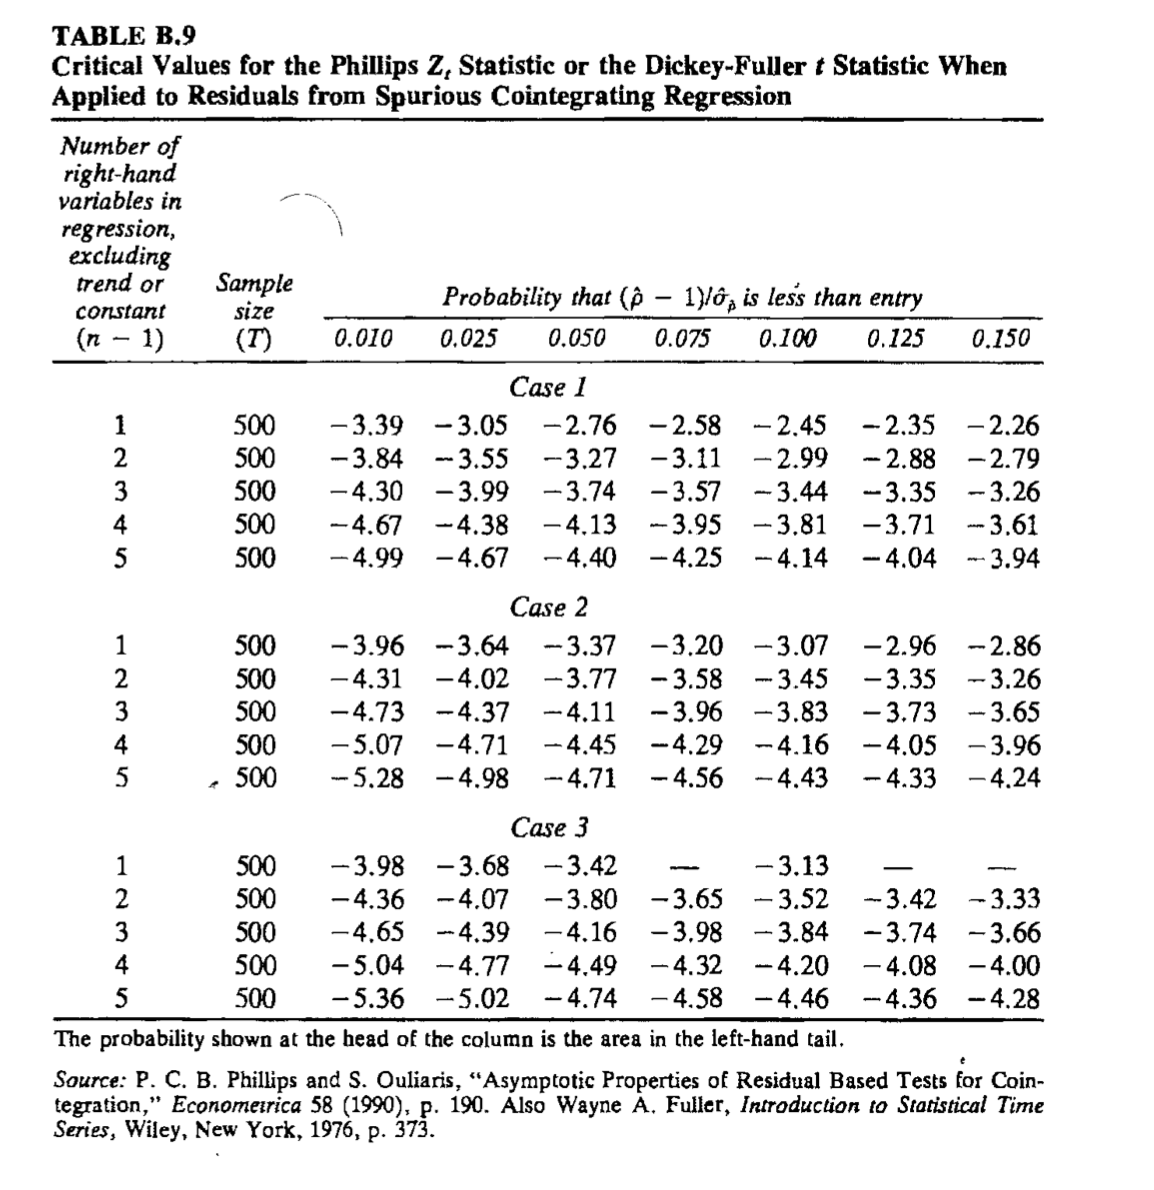
\includegraphics[scale=0.4]{graficos/tabela.png}
	\end{figure}
\end{frame}

\begin{frame}{O que o MQO estima sob cointegração?}
\begin{itemize}
	\item Para um processo vetorial $\boldsymbol{Z}_t = (y_t,\boldsymbol{x}_t)$ $n$-variado cointegrado, há no mínimo uma, e no máximo $n-1$ relações de cointegração linearmente independentes disponíveis.
	\begin{itemize}
		\item Se houvesse $n$ relações de cointegração, é possível mostrar que o processo na verdade seria estacionário.
	\end{itemize}
	\item Sejam $\left\{(1,
		\boldsymbol{b}_1'
	)', 
(1,
\boldsymbol{b}_2'
)',\ldots, (1,
\boldsymbol{b}_q'
)'\right\}$ as $q$ relações linearmente independentes que envolvem $y_t$.
		\item Se $q > 0$, possível mostrar que estimador de MQO de $y_t$ em  $\boldsymbol{x}_t$ e em um intercepto é consistente para o parâmetro $\gamma^* \in \operatorname{span} \{\boldsymbol{b}_1,\ldots, \boldsymbol{b}_q\}$ do {\color{blue}melhor preditor linear de $y_t$ em $\boldsymbol{x}_t$} definido de tal forma que:
		$$y_t = \alpha^* + \boldsymbol{x}_t '\gamma^* + u_t\, $$
		com $u_t$ estacionário, $\mathbb{E}[u_t] = 0$ e $\operatorname{cov}(\boldsymbol{x}_t,u_t) = \boldsymbol{0}$.
		\begin{itemize}
			\item Se $\operatorname{cov}(\Delta \boldsymbol{x}_t , u_s) = \boldsymbol{0}$ para todo $t$ e $s$, podemos realizar inferência sobre  $\gamma^*$ com base no estimador de MQO, estatísticas $t$ com erros padrão HAC e valores críticos normais.
		\end{itemize}
		\item Se $q=0$, inferência com base no MQO é espúria.
\end{itemize}
\end{frame}

\begin{frame}{Limitações da metodologia de Engle-Granger}
	\begin{wideitemize}
		\item Não obstante sua praticidade, a metodologia de Engle-Granger possui algumas limitações:
		\begin{itemize}
			\item Ao efetivamente escolher uma variável do lado esquerdo, nos restrigimos a relações de cointegação que envolvem $y_t$.
			\item Se $n>2$, não conseguimos separar as relações de cointegração distintas (linearmente independentes) potencialmentes existentes, cada uma correspondente a uma relação de longo prazo diferente.
			\item Além disso, para conduzir inferência sobre o vetor de cointegração estimado, necessitamos de hipóteses mais fortes sobre os erros.
		\end{itemize}
		\item Como veremos a seguir, o {\color{blue}teorema da representação de Granger} nos diz que, para um sistema de variáveis cointegrado, há restrições no processo gerador que são úteis para separar as relações de cointegração existentes.
		\begin{itemize}
			\item Essas relações podem ser usadas para construir modelos preditivos superiores (a um VAR em primeiras diferenças).
			\item Além disso, a metodologia nos permite testar hipóteses sobre as diferentes relações diretamente.
		\end{itemize}
	\end{wideitemize}
\end{frame}

\begin{frame}{Teorema de representação de Granger}
	\begin{wideitemize}
		\item Seja $\{\boldsymbol{Z}_t\}_{t\in \mathbb{Z}}$ um processo vetorial em $\mathbb{R}^n$ em que cada uma das variáveis é $I(1)$, e o processo é descrito por um VAR(p):
		
		\begin{equation}
			\boldsymbol{Z}_t = \boldsymbol{c} + \sum_{j=1}^p A_j \boldsymbol{Z}_{t-j} + \boldsymbol{v}_t \, . 
		\end{equation}
		\item {\color{blue}Teorema de representação de Granger:} $\boldsymbol{Z}_t$ é CI(1,1) se, e somente se, admite a {\color{blue}representação de correção de erros}:
		\begin{equation}
			\label{coint_system}
			\Delta \boldsymbol{Z}_t  =  \boldsymbol{c} + \boldsymbol{\alpha}'\boldsymbol{\beta} \boldsymbol{Z}_{t-1} + \sum_{j=1}^{p-1} \boldsymbol{B}_{j} \Delta  \boldsymbol{Z}_{t-j} + \boldsymbol{v}_t \, , 
		\end{equation}
		onde $\boldsymbol{\alpha}$ e $ \boldsymbol{\beta}$ são matrizes $r \times n$ com posto $r$, e cada uma das linhas de $\boldsymbol{\beta}$ corresponde a uma das $r \in \{1,\ldots, n-1\}$ relações de cointegração linearmente independentes do sistema.

	\end{wideitemize}
\end{frame}

\begin{frame}{Cointegração e correção de erros}
\begin{wideitemize}
	 		\item Teorema de representação de Granger nos diz que, se sistema é cointegrado, variações de curto prazo $\Delta \boldsymbol{Z}_t$ respondem a desvios nas $r$ relações de longo prazos, de modo a garantir a tendência comum de longo prazo do sistema.
	 		\item Do ponto de vista preditivo, o teorema nos diz que, se as variáveis são cointegradas, a relação de cointegração deve ser usada na predição (relativamente a trabalhar com um VAR em primeiras diferenças).
	 		\begin{itemize}
	 			\item Por outro lado, embora, em um sistema cointegrado, um estimador de VAR irrestrito em nível é consistente para os parâmetros populacionais (a relação não é espúria), o teorema de representação de Granger nos mostra que há restrições que podem ser incorporadas na estimação, o que pode aumentar a eficiência dos estimadores dos parâmetros.
	 		\end{itemize}
	 		\item Veremos a seguir como o modelo vetorial de correção de erros (VECM) pode ser estimado, e suas estimativas podem ser usadas para se testar o número de relações de cointegração existentes no sistema.
	 	\end{wideitemize}
\end{frame}

\begin{frame}{Detectando o número de relações de cointegração}
	\begin{itemize}
		\item Considere o estimador de máxima verossimilhança condicional de \eqref{coint_system}, onde a verossimilhança é derivada sob a hipótese auxiliar de que $\boldsymbol{v}_t \overset{iid}{\sim} N(\boldsymbol{0}_{n\times 1}, \Sigma)$, e a estimação impõe que $r=q$.
		\begin{halfwideitemize}
			\item Podemos escolher $p$ preliminarmente ajustando um VAR \textbf{em nível} e fazendo os procedimentos vistos na aula anterior.
		\end{halfwideitemize}
								\item Defina por  $\hat{L}_q$ a log-verossimilhança, no máximo atingido, calculada sob a hipótese de que $r=q$.
		\item \citet{Johansen1991} propõe testar:
		$$H_0 : r= q, \quad H_1: r= q+1\, ,$$
		usando a estatística de razão de verossimilhança $\text{LR}(q,q+1) = 2 \cdot (\max_{j \in \{q,q+1\}} \hat L_{j} - \hat L_q)  = 2 \cdot ( \hat L_{q+1} - \hat L_q)$.
		\begin{itemize}
			\item Distribuição não padrão sob a nula, e tabulada pelo autor.
			\item Estatística de teste conhecida como do {\color{blue}máximo autovalor}, visto que pode ser obtida através de um autovalor de uma matriz auxiliar calculada a partir dos dados.
		\end{itemize}
				
	\end{itemize}
\end{frame}
\begin{frame}{Procedimento sequencial e estatística do traço}
	\begin{itemize}
				\item Com base no teste do máximo autovalor, podemos detectar $r$ procedendo sequencialmente, começando os testes com $q=0$ e parando no momento em que não rejeitamos mais a nula.
				\begin{itemize}
					\item Valor de $r$ é dado pelo menor $q$ tal que não rejeitamos a nula do teste.
				\end{itemize} 
	 		\item Um outro teste possível é:
		$$H_0 : r= q, \quad H_1: r> q+1 \, ,$$
		que pode ser conduzido a partir da {\color{blue}estatística de traço} $\text{LR}(q,n) = \max_{n\geq j\geq q}2 \cdot ( \hat L_{j} - \hat L_q)= 2 \cdot ( \hat L_{n} - \hat L_q)$, e os valores críticos tabulados por \citet{Johansen1991} para esse caso.
		\begin{itemize}
			\item Também procedemos sequencialmente, parando no $r$ em que não rejeitamos a nula. 
		\end{itemize}
	\end{itemize}
\end{frame}

\begin{frame}{Componentes determinísticos}
\begin{itemize}
	\item Em nossa discussão, consideramos o modelo \eqref{coint_system}, em que, a princípio, $\boldsymbol{c} \in \mathbb{R}^n$ toma qualquer valor:
	\begin{itemize}
		\item Como há no máximo $r = n+1$ relações de cointegração, possível mostrar que a constante irrestrita permite $n - r> 0$ tendências lineares linearmente independentes  afetando o nível das séries; além de $r$ médias distintas em cada uma das relações de cointegração.
		\item Essa flexibilidade vem ao custo de poder reduzido.
	\end{itemize} 
	\item Se sabemos que não há tendências lineares no nível das séries, mas ainda assim queremos permitir que as relações de cointegração tenham média diferente de zero, podemos considerar o modelo: 
			\begin{equation*}
		\Delta \boldsymbol{Z}_t  = \boldsymbol{\alpha}'[\boldsymbol{a} + \boldsymbol{\beta} \boldsymbol{Z}_{t-1} ]+ \sum_{j=1}^{p-1} \boldsymbol{B}_{j} \Delta  \boldsymbol{Z}_{t-j} + \boldsymbol{v}_t \, , 
	\end{equation*}
	com $\boldsymbol{a} \in \mathbb{R}^{r}$. Ao reduzir o número de parâmetros ganhamos poder (valores críticos para os testes mudam nesse caso).
\end{itemize}
\end{frame}

\begin{frame}{Componentes determinísticos (cont.)}
	\begin{itemize}
	\item Por outro lado, se queremos considerar que a cointegração somente remove a tendência estocástica, devemos considerar o modelo:
\begin{equation*}
	\Delta \boldsymbol{Z}_t  =\boldsymbol{a}+ \boldsymbol{\alpha}'[\boldsymbol{b}t + \boldsymbol{\beta} \boldsymbol{Z}_{t-1} ]+ \sum_{j=1}^{p-1} \boldsymbol{B}_{j} \Delta  \boldsymbol{Z}_{t-j} + \boldsymbol{v}_t \, , 
\end{equation*}
\item Por fim, também é possível considerar testes nos diferentes modelos sob a presença adicional de \textit{dummies} sazonais.
	\begin{itemize}
	\item Valores críticos tabulados em \citet{Johansen1995}.
\end{itemize}
	\end{itemize}

\end{frame}

\begin{frame}{Inferência sobre parâmetros do VECM}
\begin{itemize}
	\item Estimado um VECM, podemos fazer inferência individual (conjunta) sobre  os $\boldsymbol{\beta}$ usando estatísticas $t$ ($F$) e valores críticos normais ($F$).
	\begin{itemize}
		\item Um ponto importante é que existem diferentes pares $(\boldsymbol{\alpha},\boldsymbol{\beta})$ compatíveis com $r$ relações de cointegração (linearmente independentes) $\implies$ precisamos normalizar $\boldsymbol{\beta}$ para separar $\boldsymbol{\alpha}$ de $\boldsymbol{\beta}$.
	\end{itemize}
	\item Como alternativa, é possível testar algumas nulas conjuntas sobre os $\boldsymbol{\beta}$ usando a estatística LR, sem necessidade de normalização.
\begin{itemize}
	\item Por exemplo, podemos testar que somente um subconjunto de $q \geq r$ das variáveis  participa das relações.
\end{itemize}
\item Podemos fazer inferência individual ou conjunta sobre os $\boldsymbol{B}_j$ e $\boldsymbol{\alpha}$ usando estatística $t$ ou testes $F$ convencionais, respectivamente.
\begin{itemize}
	\item Para testar $\boldsymbol{\alpha}$, precisamos de normalizações em $\boldsymbol{\beta}$, embora não seja o caso para testes que só envolvem os  $\boldsymbol{B}_j$.
\end{itemize}
	\item No entanto, \textbf{não} é possível, no geral, fazer testes de causalidade de Granger usando as distribuições convencionais de referência.
	\begin{itemize}
		\item Isso se deve à nula envolver restrições sobre coeficientes associados a variáveis I(0) e I(1) $\implies$ falha de aproximações convencionais.
	\end{itemize}
\end{itemize}
\end{frame}

\begin{frame}{Metodologia VAR com séries I(1)}
\begin{itemize}
	\item A discussão anterior sugere o seguinte procedimento para se ajustar um VAR com séries I(1).
	\begin{enumerate}
		\item Checar pela presença de cointegração. 
		\item Se não há cointegração ($r=0$), estimar um VAR(p-1) em primeiras diferenças.
		\begin{itemize}
			\item Nesse caso, inferência tradicional é válida para todos os parâmetros estimados.
		\end{itemize}
		\item Se há cointegração ($r>0$), estimar o modelo de correção de erros, impondo o número de relações de cointegração detectadas.
		\begin{itemize}
			\item Nesse caso, é possível fazer inferência como discutido no slide anterior.
		\end{itemize}
	\end{enumerate}

\end{itemize}
\end{frame}
\begin{frame}{VAR(p) em nível com séries I(1)}
\begin{itemize}
	\item Embora seja possível mostrar que, com séries I(1), o estimador do VAR(p) em nível seja consistente para os parâmetros tanto com $r=0$ como com $r>0$, há dois motivos para não fazê-lo.
	\item Estimar um VAR(p-1) em primeira diferença quando $r=0$ é preferível do ponto de vista de eficiência estatística, visto que efetivamente restringimos os coeficientes da representação VECM equivalentepea.
\item Além disso, estimar o VAR(p-1) em primeira diferença quando $r=0$ ou a representação VECM quando $r>0$ é peferível à estimação direta VAR(p) em nível, visto que temos garantias de inferência válida para diferentes subconjuntos dos parâmetros.
\begin{itemize}
	\item De modo geral, inferência no VAR(p) em nível não é padrão em nenhum dos casos.
\end{itemize}

\end{itemize}
\end{frame}
\begin{frame}{Metodologia VAR com séries I(0) e I(1)}
	\begin{itemize}
		\item E se há as variáveis de interesse envolvem processos I(1) e I(0)?
	\begin{itemize}
		\item Nesse caso, comumente se estima um VAR com as séries I(1) em primeiras diferenças, e as séries I(0) em nível.
		\begin{itemize}
					\item No entanto, isso ignora a possível cointegração entre as séries I(1).
		\end{itemize}
	\item Uma alternativa é detectar as $r$ relações de cointegração entre as séries I(1), e, se $r>0$, estimar um VECM com $r+n_0$ relações de cointegração, onde $n_0$ é o número de variáveis I(0).
	\begin{itemize}
		\item Recorde-se que, numa representação VECM com $s$ variáveis, se há $s$ relações de cointegração, os processos são efetivamente estacionários.
			\item Se $r=0$, estimamos o VAR misto, com as séries I(1) em diferença e as I(0) em nível.
	\end{itemize}

	
\end{itemize}
\end{itemize}
\end{frame}
\appendix
\begin{frame}[allowframebreaks]{Referências}
	\printbibliography
\end{frame}
\end{document}

